\chapter{Model-Free Deep Hedging of Variable Annuities}

\section{Introduction}

Reinforcement Learning (RL) is a branch of machine learning that focuses on training algorithms, known as agents, to make a sequence of decisions. 
The agent learns to achieve a goal in an uncertain, potentially complex environment by trial and error, using feedback from its own actions and experiences. 
Unlike supervised learning, where training data is labeled with the correct answers, in RL, an agent is provided with rewards or punishments as signals for its actions.

The core of RL revolves around the concept of the agent interacting with its environment over time, aiming to maximize the cumulative reward. 
This process involves observing the state of the environment, selecting and performing actions, and receiving rewards or penalties in response to those actions. 
The agent's objective is to learn a mapping from states to actions that maximizes this cumulative reward, which is often referred to as a policy. 
One of the fundamental frameworks for modeling RL problems is the Markov Decision Process (MDP). 
An MDP provides a mathematical formulation of the decision-making process, characterized by states, actions, rewards, and transition probabilities. 
Solving an MDP involves finding a policy that maximizes some function of the expected rewards, typically the expected cumulative reward over time.

RL algorithms can be broadly categorized into two types: model-based RL and model-free RL. 
Model-based RL utilize a model of the environment to simulate the outcomes of actions, enabling planning and decision-making with fewer interactions with the environment. 
The biggest drawback of model-based RL is model bias. 
In practice, the ground-true model is usually not available.
By using a model, an RL agent can exploit the model bias, which leads to suboptimal performance in the real environment.
Conversely, model-free RL learn directly from interactions with the environment.
Without relying on a model, model-free RL algorithms are more straightforward implement and tune.

A compelling application of RL is dynamic hedging, where the complexity and uncertainty of financial markets make traditional static models inadequate.
RL's adaptability and learning capabilities offer a promising solution to dynamically adjust hedging strategies in response to market movements and assumptions changes.
In particular, model-free RL has the potential to enhance risk management practices by developing robust strategies that can adapt in real-time.
Some popular RL algorithms include Proximal Policy Optimization (PPO), Deep Q-Networks (DQN), and Deep Deterministic Policy Gradient (DDPG).

In this paper, we propose a model-free RL algorithm to improve the risk management of variable annuities (VAs).
VAs are popular insurance products that add investment features to an insurance contract.
Hedging VAs is particularly challenging due to multiple sources of risk.
Our model-free RL approach aims to learn a hedging policy without directly accessing models of the underlying risk factors.
By interacting with an enviornment, the hedging policy can effectively manage the risks of VAs in a changing market environment.

The rest of the paper is organized as follows: 

\section{Markov Decision Process}

An MDP is defined by the tuple $\mathcal{M} = (\mathcal{S}, \mathcal{A}, \mathcal{P}, \mathcal{R}, \gamma)$, where:

\begin{itemize}
    \item $\mathcal{S}$ is a finite set of states.
    \item $\mathcal{A}$ is a finite set of actions.
    \item $\mathcal{P}$ is a state transition probability distribution, where $\mathcal{P}(s_{t}|s_{t-1}, a_{t-1})$ represents the probability of transitioning from state $s_t$ to state $s_{t-1}$ due to action $a_{t-1}$.
    \item $\mathcal{R}$ is a reward distribution, $\mathcal{R}(s, a, s')$ is the reward received after transitioning from state $s$ to state $s'$ due to action $a$.
    \item $\gamma$ is a discount factor, $\gamma \in [0,1]$,  which models the present value of future rewards.
\end{itemize}

The objective in an MDP is to find a policy, $\pi: \mathcal{S} \rightarrow \mathbb{P}(\mathcal{A})$, that maximizes the cumulative reward over time.
A Markov Decision Process (MDP) provides a mathematical framework for solving sequential decision-making tasks in an enviornment where outcomes are partly random and partly under the control of a hedging agent. 
For hedging VAs, the asset dynamics and the mortality model are not controlled by the agent, but the agent controls the cumulative reward by deciding on the hedging weights.
In this section, we reformulate the hedging enviornment of VAs from Section~\ref{subsec:VApayout} as an MDP and define the key components of the MDP.

\subsection{Hedging Environment of Variable Annuities} \label{subsec:VASimulation}

Consider a generic VA contract with maturity $T>0$ periods, e.g., $T=240$ months.
Then the contract expires at $T'=\min\{T,\tau\}$, i.e., the earlier of the contract maturity and the death of the policyholder.
Let $S_t$, $F_t$, and $G_t$ be the indexed stock price, the subaccount value and the guarantee value, respectively, at time $t=1,2,\ldots,T$.
Evolution of the subaccount value and the guarantee value of a VA contract affect the contract payout.
For clarity, we use $F_t$ and $F_{t_+}$ to denote the sub-account value just before and just after the withdrawal at time $t$, if any.
Let $\eta_g$ be the gross rate of management fee that is deducted from the fund value at each period and let $\eta_n < \eta_g$ be the net rate of management fee income to the insurer.
The difference between the gross management fee and the net management fee income represents the incurred investment expenses.

At the inception of the contract, i.e., $t=0$, we assume that the whole premium is invested in the stock index and the guarantee base is set to the sub-account value:
\begin{equation*}
    S_0=F_0=G_0.
\end{equation*}
At each time $t=1,\ldots,T$, the following events take place in the following order:
\begin{enumerate}
    \item The dynamic lapse rate $q_t$ is applied to the contract, i.e., $q$ of the policyholders leave the contract at time $t$.
        \begin{equation} \label{eq3:lapse}
            q_t = q_t^B \cdot \text{clip} (M_q (\frac{G_{t-1}}{F_{t-1}} - D_q), L_q, U_q),
        \end{equation}
    where $q_t^B$ is the base lapse rate, $\text{clip}(x, a, b)$ is a function that clips the value of $x$ to be within the range $[a, b]$, and $M_q$, $D_q$, $L_q$, and $U_q$ are the model parameters taken from National Association of Insurance Commissioners’ (NAIC) Valuation Manual 21~\citep{naic2021}.
    \item The sub-account value changes according to the growth of the underlying stock and the (gross) management fee is deducted. That is, 
        \begin{equation} \label{eq3:subaccount}
            F_t = F_{(t-1)_+}\cdot\frac{S_{t}}{S_{t-1}}\cdot(1-\eta_g)\cdot(1-q_t),
        \end{equation} 
    where $(x)^+=\max\{x,0\}$ and $F_{(t-1)_+}$ will be defined later. The insurer's income at time $t$ is the net management fee, i.e., $F_t\eta_n$. 

    \item The guarantee value ratchets up (ratcheting is a common feature in GMWB) if the sub-account value exceeds the previous guarantee value, i.e., 
        \begin{equation} \label{eq3:guarantee}
            G_t = \max\{G_{t-1}\cdot(1-q_t),F_t\}.
        \end{equation} 
    A GMMB can be modeled with $G_t = G_{t-1}\cdot(1-q_t)$.

    \item The withdrawal is made (for GMWB) and is deducted from the sub-account value, i.e., 
        \begin{equation} \label{eq3:withdrawal}
            F_{t_+} = (F_t - I_t)^+,
        \end{equation} 
    where $I_t = \xi G_t$. A GMMB can be modeled with $\xi = 0$.
\end{enumerate}

Consider a VA contract whose delta hedge portfolio at any time~$t$, $t=0,1,\ldots,T-1$, consists of $\Delta_t$ units in the underlying stock and $B_t$ amount of a risk-free zero-coupon bond maturing at time $T$.
The value of the hedge portfolio at time~$(t-1)$ is:
\begin{equation*}
    H_{t-1} = \Delta_{t-1} S_{t-1} + B_{t-1},
\end{equation*}
where $S_t$ is the underlying stock price and any time $t>0$.
This hedge portfolio is brought forward to the next rebalancing time~$t$, when its value becomes:
\begin{equation*}
    H_{t}^{bf} = \Delta_{t-1} S_{t} + B_{t-1}e^{r}.
\end{equation*}
Therefore, the time~$t$ hedging error, i.e., the cash flow incurred by the insurer due to rebalancing at time~$t$, is
\begin{equation}
    HE_t = H_t - H^{bf}_t, \quad t=1,\ldots, T-1.
\end{equation}
The P\&L of the VA contract includes the cost of the initial hedge ($H_0$), the hedging errors~\eqref{eq2:hedgingerror}, the unwinding of the hedge at maturity ($H^{bf}_T$), and the contract payout at time~$t\in \{0,\ldots,T\}$.
Mathematically, the present value of the liability for a GMMB contract is 
\begin{align} \label{eq3:lossGMMB}
L   & = H_0 - e^{-rT} H^{bf}_T + \sum_{t=1}^{T-1} e^{-rt} HE_t + \sum_{t=1}^T e^{-rt} C_t(\Delta_{t-1}) - \sum_{t=1}^T e^{-rt} F_t\eta_n + e^{-rT} (G_t - F_t)^+  \nonumber \\ 
    & = e^{-rT} (G_T - F_{T^+})^+ + \sum_{t=1}^T e^{-rt}  \left( \Delta_{t-1} (S_{t-1} - e^{-r} S_t) + C_t(\Delta_{t-1}) - F_t\eta_n \right) 
\end{align}
where the equality holds by a rearrangement of terms and a telescopic sum simplification of $e^{-rt}B_t$, $t=0,\ldots,T-1$, and $C_t(\Delta_{t-1}) := C \cdot S_{t-1} \cdot (|\Delta_{t-1}| + 0.01 \Delta_{t-1}^2)$ is the tranaction cost at time $t$~\cite{garleanu2013dynamic}.
Hence, the present liability consist of the hedging errors, the transaction costs, the net management fees, and the contract payouts.
Similarly, the present value of the liability for a GMWB contract is
\begin{equation} \label{eq3:lossGMWB}
L = \sum_{t=1}^T e^{-rt}  \left( \Delta_{t-1} (S_{t-1} - e^{-r} S_t) + C_t - F_t\eta_n \right)
\end{equation}
The GMWB payout is implicitly included in $F_t\eta_n$.
Both Equation~\ref{eq3:lossGMMB} and Equation~\ref{eq3:lossGMWB} neglect the transaction cost to liquidate the hedge portfolio at maturity.
The discrete-time hedging problem of VAs can be conveniently formulated as an MDP, where the states, actions, transition probabilities, policies, and rewards are defined as follows.

\subsection{State Space}

The state space $\mathcal{S}$ represents all the information needed to characterize the hedging environment.
In a VA hedging problem, $\mathbf{s}_t$, the information available to a hedging agent at each time $t$ is 
$$\mathbf{s}_t := (S_t, F_t, G_t, \tau, \Delta_{t-1}) \in \mathcal{S}.$$
where $\tau$ is the remaining time to maturity and $\Delta_{t-1}$ is the previous hedging weight.
The hedging environment is partially observed, e.g., the agent does not have access to the contract specifications.
It has to learn a representation of the relevant information from the observed state $\mathbf{s}_t$.

\subsection{Action Space}

The action space $\mathcal{A}$ represents the set of actions that the agent can take at each time $t$.
In a VA hedging problem, the action space only includes the hedging weight $\Delta_t$.

\subsection{Policy}

A policy $\pi$ determines the best action to take in a given state, i.e.,
$$a_t \sim \pi(\cdot|\mathbf{s}_t).$$
In a VA hedging problem the policy outputs the hedging weight $a_t = \Delta_t$ given the observed state $\mathbf{s}_t$.
In the following sections, we will refer to $\Delta_t$ as the policy.

\subsection{Transition Probabilities}

The transition probabilities $\mathcal{P}$ represent the probability of transitioning from one state to another from taking an action.
In our setup, the transition probabilities are fully determined by Equation~\ref{eq3:lapse}, Equation~\ref{eq3:subaccount}, Equation~\ref{eq3:guarantee}, and Equation~\ref{eq3:withdrawal}.
Let $\mathcal{P}(\mathbf{s}_{t+1}|\mathbf{s}_t, a_t)$ be the probability of transitioning from state $\mathbf{s}_t$ to state $\mathbf{s}_{t+1}$ due to action $a_t$.
Aside from the previous hedging weight $\Delta_{t-1}$, the transition probabilities are independent from the actions.
Paths simulated from the transition probabilities are called trajectories (or episodes) of the MDP.

\subsection{Reward and Discount Factor}
The reward function $\mathcal{R}$ and discount factor $\gamma$ in a typical RL problem are defined as follows:
\begin{align}
    \mathcal{R} & = \sum_{t=1}^{T-1} \gamma^t R_t \\
    \gamma      & = e^{-r}, \nonumber
\end{align}
where $R_t$ is the term reward received by the agent at time $t$, and the discount factor $\gamma$ is conveniently inherited from the risk-free rate $r$. 
In hedging, the term reward $R_t$ should be drived from Equation~\ref{eq3:lossGMMB} and Equation~\ref{eq3:lossGMWB} to represent the performance of the hedging policy, i.e., how closely the hedging portfolio tracks the liability.
For GMWB, we propose a term reward formulation that encourages the agent to maximize the expected reward with low hedging errors and transaction costs:
\begin{equation} \label{eq3:rewardGMWB}
    R_t = F_{t-1}\eta_n - \Delta_{t-1} |S_{t-1} - e^{-r}S_{t}| - C_{t-1}(\Delta_{t-1}), \quad t \in \{1,\ldots,T \}
\end{equation}
The reward function of GMWB directly links to the time-$t$ loss of a GMWB contract as in Equation~\ref{eq3:lossGMWB}.
The GMMB loss consists of an additional payoff at maturity $T$, thus its term reward is formulated as:
\begin{equation} \label{eq3:rewardGMMB}
    R_t = 
    \begin{cases}
    F_{t-1}\eta_n - \Delta_{t-1} |S_{t-1} - e^{-r}S_{t}| - C_{t-1}(\Delta_{t-1}),                         & t\in \{1,\ldots,T-1 \} \\
    F_{t-1}\eta_n - \Delta_{t-1} |S_{t-1} - e^{-r}S_{t}| - C_{t-1}(\Delta_{t-1}) + (G_T - F_{T^+})^+      & t = T
    \end{cases}
\end{equation}
It is worth noting that learning to hedge GMWB is easier for an RL agent due to the absense of reward at maturity (long-term feedback).

\subsection{Value Function and Advantage Function}

This section introduces some critical concepts in RL, i.e., the value function and the advantage function.
They are essential for understanding the performance of the hedging policy and the learning process of the RL agent.

A value function quantifies the expected cumulative reward over time.
The state value function, $V^{\pi}(s_t)$, is defined as the expected cumulative reward starting from state $s_t$ and following policy $\pi$ thereafter:

\begin{equation} \label{eq3:V_pi}
    V^{\pi}(s_t) = \mathbb{E} \left[ \sum_{t=0}^{\infty} \gamma^t R_t |\pi, s_t \right],
\end{equation}

where $R_t$ is the reward received by the agent after taking action $a_t$ in state $s_t$ and transitioning to state $s_{t+1}$, and the expectation is taken over the possible sequences of states and rewards that follow from the policy $\pi$.
The state-action value function, $Q^{\pi}(s_t, a_t)$, is defined as the expected cumulative reward starting from state $s_t$, taking action $a_t$, and following policy $\pi$ thereafter:

\begin{equation} \label{eq3:Q_pi}
    Q^{\pi}(s_t, a_t) = \mathbb{E} \left[ \sum_{t=0}^{\infty} \gamma^t R_t |\pi, s_t, a_t \right],
\end{equation}

Based on Equations~\ref{eq3:V_pi} and~\ref{eq3:Q_pi}, the advantage function, $A^{\pi}(s_t, a_t)$, is defined as the difference between the state-action value function and the state value function:

\begin{equation} \label{eq3:A_pi}
    A^{\pi}(s_t, a_t) = Q^{\pi}(s_t, a_t) - V^{\pi}(s_t).
\end{equation}

The advantage function quantifies the advantage of taking action $a_t$ in state $s_t$ over following the policy $\pi$.

\section{Model-Based and Model-Free RL}

\subsection{Model-Based RL: From AlphaZero to Deep Hedging}
Deep reinforcement learning first attacted attentions when AlphaGo~\citep{silver2016mastering} surpasses human in playing Go. 
Soon after, AlphaZero~\citep{silver2016mastering} emerged as a model-based RL algorithm that improves over self-plays.
It quickly extended beyond Go to other games like Chess and Shogi.
In essence, the AlphaZero agent use a neural network to paramaterize the policy and the value function.
The neural network takes the current state of the game as input and outputs the probability distribution of the next move and a value of the current state.
\begin{equation}
    (\mathbf{\pi}, v) = f_{\theta}(s), \quad L(\theta) = - \mathbf{\pi}^{\intercal} \log(\mathbf{p}) + (z - v)^2  + c||\theta||^2,
\end{equation}
where $f_{\theta}$ is the neural network with parameters $\theta$, $s$ is the current state of the game, $\pi$ is the policy, $v$ is the value of the current state, and $c$ is a regularization parameter.
$\mathbf{p}$ and $z$ are the probability distribution of the next move and the outcome of the game, respectively.
They are induced by a planning algorithm, i.e., Monte Carlo Tree Search (MCTS).
Since it is infeasible to efficiently simulate trajectories in the game of Go, a planning algorithm is necessary to generate expected outcomes.
The neural network $f_{\theta}$ is trained with a stochastic gradient descent algorithm to minimize $L$.
$L$ has three components.
The last term penalizes large neural network weights.
Its first two terms measure the similarity between $f_{\theta}(s)$, the learned policy and value function, with the action and game outcome planned by the MCTS.
The neural network is trained to predict the outcome of the game and the next move before they are actually observed.
This is known as model-based RL~\citep{sutton2018reinforcement}.
Using a model allows for planning, i.e., decision-making take place using future situations that have not been experienced by the agent.

In a typical hedging problem, the transition probabilities are independent from the hedging weights, i.e., the actions.
This simplifies the planning of the neural network as complete trajectories can be simulated without the need of a planning algorithm.
In contrast to AlphaZero, deep hedging~\citep{buehler2019deep} only uses $f_{\theta}$ for planning.
More specifically, at any time $t$, the neural network $f_{\theta}$ serves as a model that predict possible future rewards before they are actually observed.
Let $(\tilde{\mathbf{s}}_0, \tilde{\Delta}_0, \tilde{\mathbf{s}}_1, \tilde{\Delta}_1, \ldots, \tilde{s}_T)$ and $\tilde{\mathcal{R}} = (R_1, \ldots, R_t)$ be a trajectory and the hedging reward of the MDP, respectively.
The neural network $f_{\theta}$ takes the previous state and hedging weight as input and outputs the hedging weight at the current state.
\begin{equation} \label{eq3:deephedging}
    \mathbf{\Delta} = f_{\theta}(\mathbf{s}_0, \ldots, \mathbf{s}_T), \quad L(\theta) = \rho(L) = \rho(-\mathcal{R}) = \rho(- \sum_{t=0}^{T} \gamma^t R_t),
\end{equation}
where $\rho(L)$ is a convex risk measure of the total present liability $L$. 
A common choice of $\rho$ is a CVaR.
In practice, the neural network $f_{\theta}$ is trained to minimize the empirical CVaR over a batch of trajectories.
It serves as a model of the hedging environment which plans according to model predictions.
~\cite{xu2020variable} propose a deep hedging algorithm for VAs that falls into this category of model-based RL.
A cost function is defined to minimize the expected shortfall of the total present liability.
~\cite{carbonneau2021deep} extends the model-based approach to hedging long-term financial derivatives and compares the performance of deep hedging strategies trained with different cost functions.
In Equation~\ref{eq3:deephedging}, the state space of the MDP contains the previous hedging weight.
A more recent paper by~\cite{imaki2021no} proposes a new network architecture that removes the previous hedging weight from the state space by introducing a no-transaction band.
It allows for a more efficient training of the neural network by removing the semi-recurrent problem structure.
Despite the success of model-based RL in hedging, most studies focus on hedging different types of contracts on classical asset models, e.g., Black-Scholes model and Heston model.
Motivated by the seminal work by~\cite{gatheral2022volatility}, there are a many subsequent works focusing on roughening the classical stochastic volatility models. 
In the rough volatility models, the latent volatility process is modelled by a stochastic process that is rougher than the sample paths of diffusion process. 
Among these rough volatility models, notable examples are rough Heston model and the rough Bergomi model. 
Model-based RL struggles in a rough volatility model due to difficulties in designing a suitable cost function.~\cite{horvath2021deep} shows that a standard implementation of deep hedging can lead to suboptimal hedging performance in a discretized rough Bergomi model. 
The CVaR-based cost function needs to be redesigned to account for jump risks, and it is still an open question.
In summary, model-based RL algorithms like deep hedging do not depend on the asset model, i.e., they are \textbf{model-independent}.
However, they are not \textbf{model-free}.
For example, deep hedging builds its own model of the hedging environment to plan the hedging strategy ahead of time using a neural network.
Designing a suitable cost function for such a network is necessary but challenging.
In contrast, a model-free approach does not require a explicit design for different asset dynamics, making it more flexible and adaptable to different market conditions and more robust to model misspecification.

\subsection{Model-Free RL for Hedging}
    
In a model-free reinforcement learning approach, the agent is a trial-and-error learner that interacts with the environment to learn the optimal policy by iteratively updating the policy and the value function based on the observed states, actions, and rewards.
For hedging VAs, the agent does not have access to a planning algorithm or a model of the underlying risk factors, and it must learn the optimal policy by directly interacting with the environment.
Boardly speaking, model-free RL can be categorized into two types: value-based RL and policy-based RL.
Value-based approaches learn the value function directly from the data and derive the policy from the learned value function. 
The value function is learned by training a DNN to approximate the value function, which quantifies the expected cumulative reward over time. 
The policy is then derived from the learned value function by selecting the action that maximizes the value function at each state. 
~\cite{mnih2015human} is the first paper to demonstrate the effectiveness of value-based deep reinforcement learning in training agents to play Atari games.
To update the value function, the DNN is trained to minimize the difference between the current value function and the target value function, which is updated based on the maximum expected reward from the previous iteration.
When trained to approximate the value function, the DNN benefits from the use of experience replay buffers, which is proposed by~\cite{lin1992self} to store and sample historical transitions and uniformly sampled during training to enhance the sample efficiency and stability of the learning process.
~\cite{kolm2019dynamic} uses a value-based deep reinforcement learning approach to hedge European options under the Black-Scholes framework.

In valued-based approaches, the value function is updated iteratively with the maximum expected reward of all possible actions, which can be computationally expensive for continuous action spaces.
To overcome this difficulty, a policy-based approach estimates the value function before realization of the final payoff of the hedging portfolio, which is particularly useful for hedging long-term financial derivatives or VA contracts.
Two types of policy-based approaches prevail in the literature: actor-critic and policy gradient methods.

An actor-critic method designs an actor network and a critic network to learn the value function and the policy simultaneously.
The actor network learns the policy by directly outputting the action based on the current state, while the critic network learns the value of an action by approximating the expected cumulative reward over time following the actor's policy.
A popular actor-critic algorithm is the Deep Deterministic Policy Gradient (DDPG) algorithm proposed by~\cite{lillicrap2015continuous}, which is implemented by~\cite{xu2022delta} in hedging financial derivatives in S\&P 500 and DJIA index options.

A policy gradient method uses policy gradient theorem to update the policy by performing gradient ascent with respect to the policy parameters.
Representative algorithms include the Trust Region Policy Optimization (TRPO) algorithm proposed by~\cite{schulman2015trust} and the Proximal Policy Optimization (PPO) algorithm proposed by~\cite{schulman2017proximal}.
~\cite{du2020deep} show that the PPO algorithm is more sample efficient and stable than the value-based approaches in training agents to hedge financial derivatives.
The most relevant paper to our study is~\cite{chong2023pseudo}, which uses the PPO algorithm to hedge GMMB with a GMDB rider under the Black-Scholes framework.
However, information of the underlying risk factors is leaked to the agent, which makes their study pseudo-model-free.
To further improve the risk management of VAs under rough volatility models, we propose a model-free deep reinforcement learning approach to hedge VAs without explicit or implicit knowledge of the underlying risk factors.

\section{Hedging VAs with a PPO Agent}
In a hedging problem, an insurer aims to find a policy $\pi$ that maximize the expected reward over time.
In a policy-based RL approach like the PPO, both the policy and the value function are parameterized by deep neural networks.
We denote the policy by $\pi_{\theta}$ and the value function by $V_{\phi}$, where $\theta$ and $\phi$ are the parameters of the value network and the policy network, respectively.
The policy is updated according to an objective function that reflects the advantage of taking action $a_t$ in state $s_t$ over following the policy $\pi$.
\begin{align}
    \max_{\theta} \mathbb{E}\left[ \min \left\{ \Lambda_t(\theta)\hat{A}^{\pi_{\theta}}(s_t, a_t), \text{clip}(\Lambda_t(\theta), 1-\epsilon, 1 + \epsilon) \hat{A}^{\pi_{\theta}}(s_t, a_t)  \right\} \right] \\
    \Lambda_t(\theta) = \frac{\pi_{\theta}(a_t|s_t)}{\pi_{\theta_{old}}(a_t|s_t)} 
\end{align}

where $\theta_{old}$ denotes the policy parameters at the previous iteration, $\epsilon$ is a clip range hyperparameter that controls the size of the policy update, $\text{clip}(x, a, b)$ is a function that clips the value of $x$ to be within the range $[a, b]$, and $\hat{A}^{\pi_{\theta}}(s_t, a_t)$ is the estimated advantage of taking action $a_t$ in state $s_t$ over following the policy $\pi_{\theta_{old}}$.
In our implementation, the advantage function is estimated following the GAE method proposed by~\cite{schulman2015high}.
The policy is updated by performing gradient ascent with respect to the policy parameters $\theta$ to maximize the objective function, which is estimated by sampling from the environment and computing the empirical average of the objective function over the sampled trajectories.
The first component in the objective function, $\Lambda_t(\theta) \hat{A}^{\pi_{\theta}}(s_t, a_t)$, is a surrogate objective function that approximates the advantage of taking action $a_t$ in state $s_t$ over following the policy $\pi_{\theta_{old}}$, and the second component, $\text{clip}(\Lambda_t(\theta), 1-\epsilon, 1 + \epsilon) \hat{A}^{\pi_{\theta}}(s_t, a_t)$, is a clipped surrogate objective function that prevents large policy updates and ensures more stable training.
The TRPO algorithm proposed by~\cite{schulman2015trust} uses a similar clipped surrogate objective function to ensure that the policy update does not deviate too far from the old policy, but PPO simplifies the optimization problem by using a clipped surrogate objective function instead of a hard-coded constraint on the policy update.
Compared to TRPO, PPO is more computationally efficient and easier to implement, making it a popular choice for training deep reinforcement learning agents.
For a in-depth discussion on the implementation details of both TRPO and PPO, we refer the reader to~\cite{engstrom2020implementation}.

\begin{algorithm} 
    \caption{PPO for Hedging Variable Annuities} 
    \begin{algorithmic}[1] \label{alg3:ppoHedging}
        \STATE  Initialize policy parameters $\theta_0$ and value function parameters $\phi_0$.
        \STATE  \textbf{For} {iteration $k=0, 1,2,\ldots$} \textbf{do}
        \STATE  \quad Collect a set of trajectories $\mathcal{D}_k$ by sampling from the environment with policy $\pi_{\theta_{k}}$.
        \STATE  \quad Compute the rewards $\hat{R}_t$ for each trajectory in $\mathcal{D}_k$.
        \STATE  \quad Estimates the advantage function with $\hat{A}_{\pi_{\theta_k}}(\mathbf{s}_t, a_t)$ using value function $V_{\phi_k}$.
        \STATE  \quad Update the policy parameters $\theta_{k+1}$ by 
        \begin{equation*}
            \max_{\theta} \mathbb{E}\left[ \min \left\{ \Lambda_t(\theta)\hat{A}^{\pi_{\theta}}(\mathbf{s}_t, a_t), \text{clip}(\Lambda_t(\theta), 1-\epsilon, 1 + \epsilon) \hat{A}^{\pi_{\theta}}(\mathbf{s}_t, a_t)  \right\} \right]
        \end{equation*}
        \STATE  \quad Update the value function parameters $\phi_{k+1}$ by minimizing the mean squared error between the predicted value and the actual collected reward.
        \begin{equation*}
            \phi_{k+1} = \arg \min_{\phi} \frac{1}{|\mathcal{D}_k|T} \sum_{\mathcal{\kappa} \in \mathcal{D}_k} \sum_{t=0}^{T} \left( V_{\phi}(\mathbf{s}_t) - \hat{R}_t \right)^2
        \end{equation*}
        \STATE  \textbf{End For}
    \end{algorithmic}
\end{algorithm}

Algorithm~\ref{alg3:ppoHedging} outlines the PPO algorithm for training an agent to hedge VAs.
At each iteration $k$, the agent collects a set of trajectories $\mathcal{D}_k$ by interacting with the environment (Section~\ref{subsec:VASimulation}) with the current policy $\pi_{\theta_k}$.
The agent then computes the rewards $\hat{R}_t$ for each trajectory in $\mathcal{D}_k$ and estimates the advantage function with $\hat{A}_{\pi_{\theta_k}}(s_t, a_t)$ using the value function $V_{\phi_k}$.
The policy parameters $\theta_{k+1}$ are updated by performing gradient ascent with respect to the policy parameters to maximize the clipped surrogate objective function.
The value function parameters $\phi_{k+1}$ are updated by minimizing the mean squared error between the predicted value and the actual collected reward.
The agent iterates this process until convergence to learn an optimal policy for hedging VAs.

\subsection{Accounting for Non-Markovian Dynamics}

In the context of hedging VAs, the state space is partially observed.
The agent does not have access to the contract specifications and the underlying risk factors.
Furthermore, a rough volatility model introduces non-Markovian dynamics, i.e., the future state of the system depends on the entire history of the system.
To address the non-Markovian dynamics, an LSTM component is added to the state representation $\mathbf{s}_t$ to capture the temporal dependencies in the data.
This approach is known as recurrent PPO~\citep{ni2021recurrent}.
Let $h_t$ be the hidden state of the LSTM at time $t$.
The state representation $\mathbf{s}_t$ with recurrent PPO is defined as:
\begin{equation} \label{eq3:stateRNN}
    \mathbf{s}_t = (S_t, F_t, G_t, \tau, \Delta_{t-1}, h_t)
\end{equation}
The policy and reward function remain the same but with the new state representation in Equation~\ref{eq3:stateRNN}.
Instead of following the standard PPO algorithm, the agent uses the recurrent PPO algorithm to learn an optimal policy for hedging VAs.

\begin{algorithm} 
    \caption{Recurrent PPO for Hedging Variable Annuities (Not Yet Done)} 
    \begin{algorithmic}[1] \label{alg3:ppoHedging-rnn}
        \STATE  Initialize policy parameters $\theta_0$ and value function parameters $\phi_0$.
        \STATE  \textbf{For} {iteration $k=0, 1,2,\ldots$} \textbf{do}
        \STATE  \quad Collect a set of trajectories $\mathcal{D}_k$ by sampling from the environment with policy $\pi_{\theta_{k}}$.
        \STATE  \quad Compute the rewards $\hat{R}_t$ for each trajectory in $\mathcal{D}_k$.
        \STATE  \quad Estimates the advantage function with $\hat{A}_{\pi_{\theta_k}}(\mathbf{s}_t, a_t)$ using value function $V_{\phi_k}$.
        \STATE  \quad Update the policy parameters $\theta_{k+1}$ by 
        \begin{equation*}
            \max_{\theta} \mathbb{E}\left[ \min \left\{ \Lambda_t(\theta)\hat{A}^{\pi_{\theta}}(\mathbf{s}_t, a_t), \text{clip}(\Lambda_t(\theta), 1-\epsilon, 1 + \epsilon) \hat{A}^{\pi_{\theta}}(\mathbf{s}_t, a_t)  \right\} \right]
        \end{equation*}
        \STATE  \quad Update the value function parameters $\phi_{k+1}$ by minimizing the mean squared error between the predicted value and the actual collected reward.
        \begin{equation*}
            \phi_{k+1} = \arg \min_{\phi} \frac{1}{|\mathcal{D}_k|T} \sum_{\mathcal{\kappa} \in \mathcal{D}_k} \sum_{t=0}^{T} \left( V_{\phi}(\mathbf{s}_t) - \hat{R}_t \right)^2
        \end{equation*}
        \STATE  \textbf{End For}
    \end{algorithmic}
\end{algorithm}

Algorithm~\ref{alg3:ppoHedging-rnn} outlines the recurrent PPO algorithm for training an agent to hedge VAs with non-Markovian dynamics.

\section{Numerical Experiments}

We present a numerical experiment to demonstrate the effectiveness of the model-free PPO algorithm for hedging VAs with transaction costs.
We consider a VA contract with a maturity of $T=240$ months and a guaranteed minimum maturity benefit (GMMB) rider with a simulation environment described in Section~\ref{subsec:VASimulation}.
The simulation enviornment is implemented in Python using the OpenAI Gym framework~\citep{brockman2016openai}, and the neural networks are programmed using the PyTorch library~\citep{paszke2019pytorch}.
The environment is designed to simulate the dynamics of the VA contract and provide the agent with the current state of the VA with the contract specifications and the financial market information described in Table~\ref{tab3:hyperparameters}.

\begin{table}[ht!]
    \centering
    \begin{tabular}{ll} 
        \toprule
        Hyperparameter      & Value \\
        \midrule
        $|\mathcal{D}_k|$   & 64        \\
        $\epsilon$          & 0.2       \\
        Learning rate       & 0.0003    \\
        $S_0$               & 1000      \\
        $\mu$               & 0.00375   \\
        $\sigma$            & 0.0457627 \\
        $r$                 & 0.002     \\
        $T$                 & 240       \\
        \bottomrule
    \end{tabular}
    \caption{PPO Hyperparameters and GMMB Contract Specifications} 
    \label{tab3:hyperparameters}
\end{table}

The underlying asset price $S_t$ is modeled as a geometric Brownian motion with a drift rate $\mu$ and a volatility $\sigma$.
The weights of the value network and the policy network are initialized with orthogonal initialization~\citep{engstrom2020implementation} with scaling $\sqrt{2}$ and the bias terms set to zero.
The value network and the policy network are implemented as fully connected neural networks with two hidden layers of 64 units each and $\tanh$ activation functions.
They are trained using the Adam optimizer with a learning rate of $0.0003$ and a batch size automatically adjusted to the number of trajectories in the collected dataset.
At each timestep, the observations are normalized and cliped between $-10$ and $10$ before being fed into the neural networks to stabilize the training process.
For PPO, we follow the suggestions in~\cite{schulman2017proximal} and set the clipping hyperparameter $\epsilon$ to $0.2$ to prevent large policy updates. 
More specifically, our implementation of the PPO uses a generalized advantage estimation~\citep{schulman2015high} to estimate the advantage function.
The agent interacts with the environment for $10^6$ episodes, and the policy and value networks are updated every $64$ episodes and evaluated every $1000$ episodes.
The performance of the agent is evaluated based on the average reward over an independent test set of $10^4$ episodes, and the results are compared with the benchmark hedging strategy, delta hedging.

\begin{figure}
    \centering
    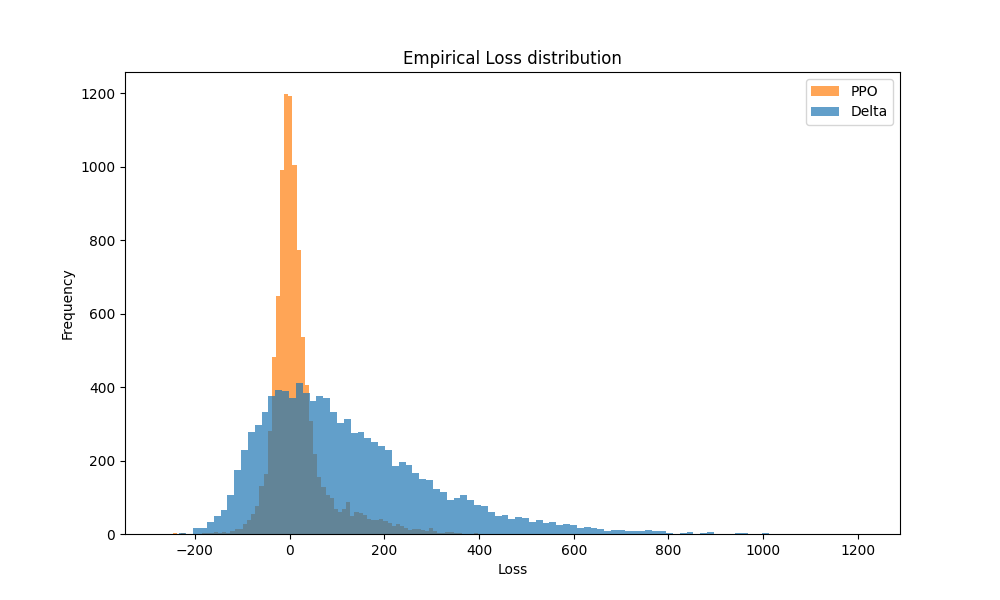
\includegraphics[width=0.8\textwidth]{./project3/figures/loss_distribution.png}
    \caption{Performance of PPO for Hedging GMMB Contracts on GBM Asset Model} 
    \label{fig3:ppo_hedging}
\end{figure}

Figure~\ref{fig3:ppo_hedging} shows the performance of the PPO algorithm for hedging GMMB contracts on a geometric Brownian motion (GBM) asset model.
The figure shows the distribution of the hedging errors incurred by the agent over the $10^4$ test episodes.
The hedging errors are calculated as the difference between the actual cash flow incurred by the agent due to rebalancing and the expected cash flow based on the optimal hedging policy.
The results show that the PPO algorithm is able to learn an optimal hedging policy that minimizes the hedging errors, and it surpasses the benchmark delta hedging strategy in terms of hedging performance.

\section{Conclusion}


